\documentclass[12pt,aspectratio=169]{beamer}

\usetheme{metropolis}

\definecolor{mDarkBrown}{HTML}{FF5722}
\definecolor{mDarkTeal}{HTML}{263238}
\definecolor{mLightBrown}{HTML}{FF5722}

\usepackage{booktabs}
\usepackage{graphicx}
\usepackage{hyphenat}
\usepackage{multirow}
\usepackage{nicefrac}
\usepackage[normalem]{ulem}

\usepackage{pifont}
\newcommand{\cmark}{\ding{51}}
\newcommand{\xmark}{\ding{55}}

\usepackage{minted}
\usemintedstyle{tango}
\newminted[bash]{bash}{%
    autogobble,
    bgcolor=mDarkTeal!10,
    linenos
}
\newminted[py3]{python}{%
    python3,
    autogobble,
    bgcolor=mDarkTeal!10,
    linenos
}
\newminted[sql]{sql}{%
    autogobble,
    bgcolor=mDarkTeal!10,
    linenos
}

\usepackage{polyglossia}
\setdefaultlanguage[variant=british]{english}
\usepackage[english=british]{csquotes}

\defaultfontfeatures{Ligatures=TeX}
\setmainfont{Lucida Sans OT}
\setsansfont[Scale=MatchLowercase]{Lucida Sans OT}
\setmonofont[Scale=MatchLowercase]{Lucida Console DK}

\usepackage{mathspec}
\setmathsfont(Digits,Latin,Greek)[Numbers={Lining,Proportional}]{Lucida Bright Math OT}

\newcommand{\mat}[1]{\ensuremath{\mathbf{#1}}}

\newcommand{\R}{\ensuremath{\mathbb{R}}}

\newcommand{\E}[1]{\ensuremath{\mathbb{E}\!\left[ #1 \right]}}
\newcommand{\V}[1]{\ensuremath{\mathbb{V}\!\left[ #1 \right]}}
\newcommand{\Prob}[1]{\ensuremath{\Pr\!\left( #1 \right)}}
\newcommand{\Normal}[2]{\ensuremath{\mathcal{N}\!\left( #1, #2 \right)}}
\newcommand{\simiid}{\ensuremath{\overset{\text{\tiny i.i.d.}}{\sim}}}

\DeclareMathOperator{\logit}{logit}

\author{Gianluca Campanella}
\date{}



\title{Introduction to Data Science}

\begin{document}

\maketitle

\begin{frame}{Contents}
    \tableofcontents[hideallsubsections]
\end{frame}

\section{What is Data Science?}

\begin{frame}{What is Data Science?}
    \begin{center}
        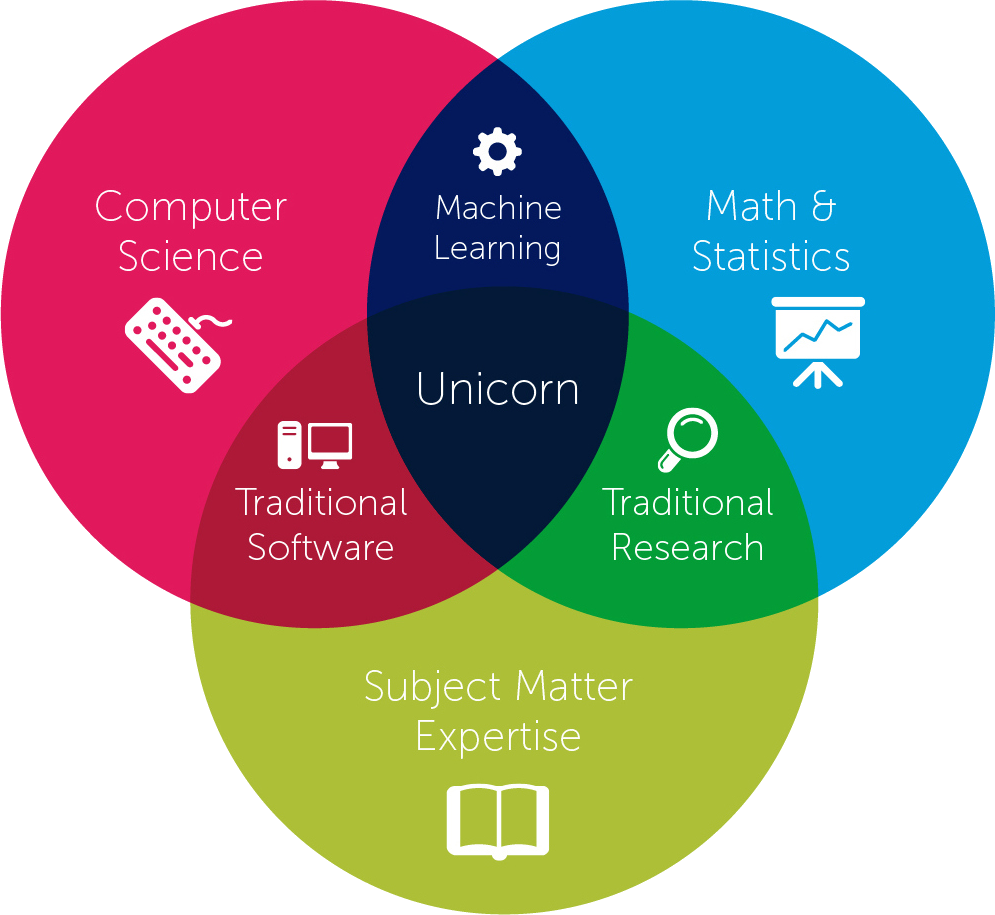
\includegraphics[height=0.8\textheight]{figures/data_science_venn_diagram} \\
        {\scriptsize%
         From S.\ Geringer (originally from D.\ Conway)}
    \end{center}
\end{frame}

\begin{frame}{How's it different from\ldots}
    \begin{block}{Statistics}\vspace{-0.25em}
        \begin{itemize}
            \item Predates computers
            \item \alert{Understand why something happens} in the face of
                  uncertainty
        \end{itemize}
    \end{block}
    \vfill\pause
    \begin{block}{Machine Learning}\vspace{-0.25em}
        \begin{itemize}
            \item `Algorithmic modelling' (L. Breiman)
            \item Computers can \alert{learn rules} without explicit programming
        \end{itemize}
    \end{block}
    \vfill\pause
    \begin{block}{Deep Learning}\vspace{-0.25em}
        \begin{itemize}
            \item Less structured inputs
            \item Computers can \alert{learn structure} without explicit
                  programming
        \end{itemize}
    \end{block}
\end{frame}

\begin{frame}{Data Science is\ldots}
    \begin{center}
        \LARGE\bf%
        Data\hyp{}driven decision\hyp{}making
    \end{center}
    \vfill
    \begin{itemize}
        \item Focus is on the problem\hyp{}solving process
        \item Multidisciplinary but domain\hyp{}centric
        \item Tools are secondary!
    \end{itemize}
\end{frame}

\begin{frame}{What does Data Science deal with?}
    \only<1>{%
        \begin{center}
            \LARGE%
            Problems!
        \end{center}
        \vfill
        Can we \alert{improve}\ldots\vspace{-1ex}
        \begin{itemize}
            \item The quality of offers we send to our customers?
            \item Road safety?
            \item How we identify people at high risk of cancer?
        \end{itemize}}
    \only<2>{%
        \begin{center}
            \LARGE%
            Predictions?
        \end{center}
        \vfill
        \alert{How likely}\ldots\vspace{-1ex}
        \begin{itemize}
            \item Is a customer to respond to some offer?
            \item Are traffic accidents to occur in a certain area?
            \item Is a person to develop cancer in the next 10 years?
        \end{itemize}}
    \only<3>{%
        \begin{center}
            \LARGE%
            Mechanisms?
        \end{center}
        \vfill
        \alert{Why}\ldots\vspace{-1ex}
        \begin{itemize}
            \item Does a customer decide to respond to some offer?
            \item Do traffic accidents occur regularly in certain areas?
            \item Do people develop cancer?
        \end{itemize}}
\end{frame}

\begin{frame}{Two types of Data Science}
    \begin{columns}
        \begin{column}{0.5\textwidth}
            \begin{center}
                \large\bf%
                Analysis\hyp{}focused
            \end{center}
            \begin{itemize}
                \item Maths and Statistics
                \item Business Intelligence
                \item[$\to$] Assist human decision\hyp{}making
            \end{itemize}
        \end{column}
        \begin{column}{0.5\textwidth}
            \begin{center}
                \large\bf%
                Building\hyp{}focused
            \end{center}
            \begin{itemize}
                \item Machine Learning
                \item Software Engineering
                \item[$\to$] Develop and deploy data\hyp{}driven products
            \end{itemize}
        \end{column}
    \end{columns}
\end{frame}

\begin{frame}{Recap}
    \begin{block}{Data Science is\ldots}
        \begin{itemize}
            \setlength{\itemsep}{0.75em}
            \item \alert{Evidence\hyp{}based problem solving and
                         decision\hyp{}making}
            \item Multidisciplinary but domain\hyp{}centric
            \item Analysis\hyp{}focused or building\hyp{}focused
        \end{itemize}
    \end{block}
\end{frame}

\section{What can Data Science do?}

\begin{frame}{The five questions}
    \begin{enumerate}
        \item How much/many?
        \item Is this A or B?
        \item How is this organised?
        \item Is this weird?
        \item What should I do next?
    \end{enumerate}
\end{frame}

\begin{frame}{How much/many?}
    \begin{block}{Examples}
        \begin{itemize}
            \item What will the temperature be next Sunday?
            \item What will total sales be next quarter?
        \end{itemize}
    \end{block}
    \begin{center}
        \large%
        $\downarrow$
        \vfill
        \alert{Regression} algorithms
    \end{center}
\end{frame}

\begin{frame}{Is this A or B?}
    \begin{block}{Examples}
        \begin{itemize}
            \item Which is more effective: a £10 voucher or a 10\% discount?
            \item Will this machine fail in the next month?
        \end{itemize}
    \end{block}
    \begin{center}
        \large%
        $\downarrow$
        \vfill
        \alert{Classification} algorithms
    \end{center}
\end{frame}

\begin{frame}{How is this organised?}
    \begin{block}{Examples}
        \begin{itemize}
            \item Which users like similar movies?
            \item Which items are frequently purchased together?
        \end{itemize}
    \end{block}
    \begin{center}
        \large%
        $\downarrow$
        \vfill
        \alert{Clustering} algorithms
    \end{center}
\end{frame}

\begin{frame}{Is this weird?}
    \begin{block}{Examples}
        \begin{itemize}
            \item Is this transaction fraudulent?
            \item Is this blood pressure reading normal?
        \end{itemize}
    \end{block}
    \begin{center}
        \large%
        $\downarrow$
        \vfill
        \alert{Anomaly detection} algorithms
    \end{center}
\end{frame}

\begin{frame}{What should I do next?}
    \begin{block}{Examples}
        \begin{itemize}
            \item Should the thermostat adjust the temperature?
            \item Where should the robot vacuum go next?
        \end{itemize}
    \end{block}
    \begin{center}
        \large%
        $\downarrow$
        \vfill
        \alert{Reinforcement learning} algorithms
    \end{center}
\end{frame}

\begin{frame}{Supervised vs unsupervised algorithms}
    \begin{columns}
        \begin{column}{0.5\textwidth}
            \begin{center}
                \large\bf%
                Supervised algorithms
            \end{center}
            \begin{itemize}
                \item Are trained on existing data
                \item Can be compared according to some `goodness' metric
            \end{itemize}
        \end{column}
        \begin{column}{0.5\textwidth}
            \begin{center}
                \large\bf%
                Unsupervised algorithms
            \end{center}
            \begin{itemize}
                \item Don't use examples with known outcomes
                \item Give clues, not `right answers'
            \end{itemize}
        \end{column}
    \end{columns}
\end{frame}

\begin{frame}{Data Science solutions}
    \begin{center}
        \begin{tabular}{lll}
            \toprule
            \textbf{Family}               & \textbf{Class}         & \textbf{Question} \\
            \midrule
            \multirow{2}{*}{Supervised}   & Regression             & How much/many? \\
                                          & Classification         & Is this A or B? \\
            \midrule
            \multirow{2}{*}{Unsupervised} & Clustering             & How is this organised? \\
                                          & Anomaly detection      & Is this weird? \\
            \midrule
                                          & Reinforcement learning & What should I do next? \\
            \bottomrule
        \end{tabular}
    \end{center}
\end{frame}

\end{document}

